%%%%%%%%%%%%%%%%%%%%%%%%%%%%%%%%%%%%%%%%%%%%%%%%%%%%%%%%%%%%%%%%%%%
%                                                                 %
%                           CHAPTER THREE                         %
%                                                                 %
%%%%%%%%%%%%%%%%%%%%%%%%%%%%%%%%%%%%%%%%%%%%%%%%%%%%%%%%%%%%%%%%%%%

\chapter{MACHINE-READABLE CHANGE LOG}\label{ch:changelog}

\section{Introduction}

Change logs explain the differences between versions; however, they are often only available in human-readable formats.
Readability puts a limit on the length and extent of the log since a human will need to write it.
Manageable change descriptions become difficult with large data sets featuring many changes, or data sets that change often, but these are exactly the data sets which need change logs the most.
Automating the process will allow more data sets to provide change documentation in a timely fashion for data sets.
Encoding the change logs with structured data will provide a means for users to efficiently consume change information.
The additional encoding will inflate the size of a standard change log which becomes an issue with the change logs.

Change logs were generated for two data sets, the ``Global Database on \textsuperscript{3}He/\-\textsuperscript{4}He in on-shore free-circulated subsurface fluids" data set and the Paragenetic Mode for Copper Minerals database.
Following the practices of other change logs, the documents present before and after values for comparison which can be seen in Figure \ref{changelog_zoomed}.
\begin{figure}
	\centering
	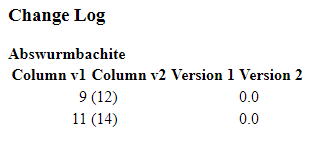
\includegraphics[scale=0.80]{figures/Changelog-zoomed.png}
	\caption{Abswurmbachite entry in the Copper Dataset Change Log}
	\label{changelog_zoomed}
\end{figure}
The change logs identify challenges to adopting thorough change logs as a practice in versioning data sets.

\section{Utilized Data Sets}

\subsection{Noble Gas Data set}

The ``Global Database on \textsuperscript{3}He/\textsuperscript{4}He in on-shore free-circulated subsurface fluids" is a tumultuous database \cite{Polyak2015}.
The first version, published in June 11, 2013, contains the information from 8 regions of the world united into a single file with around 199 columns.
The next version of the database, published March 8, 2015, reduces the number of columns to 54, marking a drastic change.
In addition, several columns changed the units with which they reported measurements.
While usage documentation, explaining the content and use of the data, accompanied each version, no records were included indicating what changed between versions.
A change log would be valuable guide with such drastic structural and content changes.
The third and most recent publication came in July 11, 2017, with no changes to the number of files or columns, but many new rows.
The structural summary of each of the files can be found in Table \ref{noble_gas_file_table}.

\begin{table}
	\caption{Files in the Noble Gas data set.}
	\label{noble_gas_file_table}
	\centering
	\begin{tabular}{|c|c|c|c|c|}
		\hline
		Filename & File Size (Bytes) & Rows & Columns &	Total Cells \\ \hline
		DB\_HE\_6733.xlsx &	2682683 &	6733 &	199 &	1339867 \\
		DB\_final-55-7262\_2015\_03 &	2729060 &	7265 &	54 &	392310 \\
		\_08.xlsx&&&&\\
		NG\_DB\_final\_2017\_07 &	4216595 &	8231 &	54 &	444474 \\
		\_01.xlsx&&&&\\
		\hline
	\end{tabular}
\end{table}

\subsection{Copper Data set}

The Paragenetic Mode for Copper Minerals database became available through collaboration with the author's lab to create new methods of visualizing mineralogy relationships \cite{Morrison2016}.
The first version was collected June 8, 2016, with the update following soon after on August 8, 2016.
Major edits are fairly limited with only 16 column additions and 2 removals between the versions.
Value formats remain consistent from one version to the next, resulting in a much more condensed body of changes, making transitions more easily verifiable.
Compared to the Noble Gas data set, it provides a more stable data platform to implement the versioning model in Section \ref{ch:model}.
The data from this work is also more processing friendly, making it agreeable to automatic change log generation.
An interesting thing to note in Table \ref{copper_file_table} is that the second version takes up less storage space even though it has more data.

\begin{table}
	\caption{Files in the Copper data set.}
	\label{copper_file_table}
	\centering
	\begin{tabular}{|c|c|c|c|c|}
		\hline
		Filename & File Size (Bytes) & Rows & Columns &	Total Cells \\ \hline
		ParageneticModeTable\_Cu\_6. &	339175 & 705 &	37 &	26085\\
		8.2016.xlsx&&&&\\
		ParageneticModeTable\_Cu\_8. & 233715 & 685 & 51 & 34935\\
		21.2016.xlsx&&&&\\
		\hline
	\end{tabular}
\end{table}

\section{Version Model Specification}\label{ch:model}

When making change logs more approachable for usage in data sets, two approaches are available.
The first approach continues writing change logs in only human readable language and relying on advances in natural language processing to allow computers to read the change logs.
The second approach uses linked data to encode the change log with machine-computable statements.
Since natural language processing is currently not sufficiently articulate, the second approach is taken.
In doing so, a versioning data model needs to be developed which can capture changes in the way a change log organizes information.

A versioning data model needs to address a variety of needs not met by provenance models.
In PROV-O and PAV, the modeled entities are exclusively one-dimensional with each version leading sequentially to the next one.
The HCLS model, Figure \ref{HCLSModel}, and Barkstrom model, Figure \ref{hierarchy}, however, display a more complex two-dimensional hierarchy.
The tree models better capture the tiered granularity separating different versions which can result from a higher-tier macro change.
These models also tightly couple new objects with changes to their underlying attributes.
The tiered approach more clearly explains the scale on which two objects within the tree differ.

Provenance models provide concepts to sequentially order data objects but lack the ability to convey differences between farther spanning objects.
In Figure \ref{hierarchy}, the left-most leaf node and the right-most leaf node differ by three changes at the data product level.
A provenance model would need to rely on qualified properties to connect further annotations and describe the higher level changes.
Remember that a common function of versioning systems is to provide a method to determine the amount of change or difference between two objects of a work.
Much of the differences become lost when compressed into a single relation in a provenance graph.
Additional annotations are often in natural language and do not provide a regular attribute to quantify.

The provenance models, on the other hand, do a much better job in explicitly defining the connection between objects which the tree models imply with structure.
The versioning model must contain a mechanism to convey how changes to parts of an object contribute to that object's transition into a new version.
The fundamental operations---\textbf{add}, \textbf{invalidate}, and \textbf{modify}---are used by the model to capture change in a more detailed manner.
These details provide a mechanism to measure change between versions with better clarity than current methods.

\subsection{Initial Approaches}

The first approach, seen in Figure \ref{DiscardedFig}, simply extends the provenance relation with additional concepts to capture more types of relationships.
\begin{figure}
	\centering
	\vspace{0.0in} % normally the command here would be \includegraphics
	%	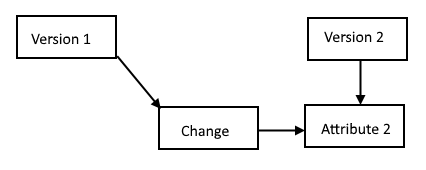
\includegraphics{figures/Addition.png}
	\begin{tikzpicture}[every node/.style={draw, rectangle}]
	\begin{scope}[node distance=10mm and 30mm]
	\node (1) [scale=1.25] at (0,0) {Version 1};
	\node (a) [below=of 1, scale=1.25] {Attribute};
	\node (p1) [below=of a, scale=1.25] {Pre-Value};
	\node (p2) [below right=of a, scale=1.25] {Post-Value};
	\node (n) [above=of p2, scale=1.25] {New};
	\node (o) [right=of n, scale=1.25] {Old};
	\node (2) [above =of o, scale=1.25] {Version 2};
	
	\draw [line width=2pt, ->] (1) -- (2);
	\draw [line width=2pt, ->] (2) -- (n);
	\draw [line width=2pt, ->] (2) -- (o);
	\draw [line width=2pt, ->] (1) -- (a);
	\draw [line width=2pt, ->] (2) -- (a);
	\draw [line width=2pt, ->] (a) -- (p1);
	\draw [line width=2pt, ->] (a) -- (p2);
	\end{scope}
	\end{tikzpicture}
	\caption{Provenance oriented versioning model.}
	\label{DiscardedFig}  % the \label command comes AFTER the caption
\end{figure}
Until the introduction of or comparison with Version 2, none of the concepts in Version 1 can be considered new or old.
As the responsible party for introducing changes, Version 2 becomes associated with New, Old, and modified attributes.
Version 1 also relates to modified attributes since it provides the pre-value used to contextualize Version 2's post-value.
The pre and post values are included so that a user can see how much the attribute has changed, much like with a change log.

Adding the attributes as concepts to the model addresses PROV's and PAV's flat approach to version relations, but the attributes do not capture the inter-relation between objects for New and Old attributes.
Having Version 2 be responsible for all the changes causes issues with the model since it must be associated with attributes from an entirely different object.
The Old attributes should not exists within Version 2.
Associating Old attributes with Version 1 would be more appropriate and intuitive to understand.
The model does not capture the type of change, making the result a listing of attributes without the version differences to contextualize the relationship between the versions.

From a different direction, Figure \ref{DiscardedFig2} shows a model created by starting from the change log.
\begin{figure}
	\centering
	\vspace{0.0in} % normally the command here would be \includegraphics
	%	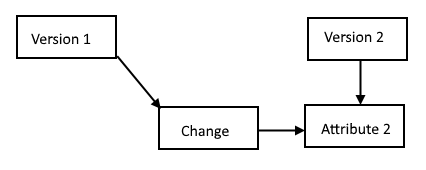
\includegraphics{figures/Addition.png}
	\begin{tikzpicture}[every node/.style={draw, rectangle}]
	\begin{scope}[node distance=10mm and 20mm]
	\node (l) [scale=1.25] at (1,0) {Log};
	\node (n) [above right=of l, scale=1.25] {New};
	\node (o) [below right=of l, scale=1.25] {Old};	
	\node (a) [right=of l, scale=1.25] {Attribute};
	\node (c) [right=of a, scale=1.25] {Change};
	\node (t) [right=of c, scale=1.25] {Type};
	\node (p1) [above right=of c, scale=1.25] {Pre-Value};
	\node (p2) [below right=of c, scale=1.25] {Post-Value};
	
	\draw [line width=2pt,->] (l) -- (n);
	\draw [line width=2pt,->] (l) -- (o);
	\draw [line width=2pt,->] (l) -- (a);
	\draw [line width=2pt,->] (a) -- (c);
	\draw [line width=2pt, ->] (c) -- (t);
	\draw [line width=2pt, ->] (c) -- (p1);
	\draw [line width=2pt, ->] (c) -- (p2);
	\end{scope}
	\end{tikzpicture}
	\caption{Change log based versioning model.}
	\label{DiscardedFig2}  % the \label command comes AFTER the caption
\end{figure}
Attributes are attached to the log as the primary indicators for old, new, and modified concepts.
Change logs often break down and group changes by attributes.
For modified attributes, an additional change concept is associated, encapsulating the values and nature of the change.
At the far right side of the figure is a concept called Type which indicates more specifically the nature of the change for example a unit of speed to another.
Pre and post values are also included to explicitly define the change concept.

The primary drawback of the log-based construction is that the change log assumes all responsibility for every modification to the data even though the document only reports the differences.
The version objects are also left out of the model, leaving the log concept in possession of the attributes.
One of the major breakthroughs with this model construction is that while specific values are kept in the log, those values do not need to be in the model.
By encoding the type of change, the need for actual values becomes superfluous as change type is more generalizable across domains and contexts.

Figure \ref{DiscardedFig3} combines the provenance and change log approaches by capturing the transition from Version 1 to Version 2 in the change log.
\begin{figure}[b]
	\centering
	\vspace{0.0in} % normally the command here would be \includegraphics
	%	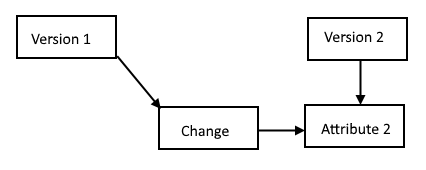
\includegraphics{figures/Addition.png}
	\begin{tikzpicture}[every node/.style={draw, rectangle}]
	\begin{scope}[node distance=10mm and 30mm]
	\node (l) [scale=1.25] at (0,0) {Log};
	\node (1) [left=of l, scale=1.25] {Version 1};
	\node (2) [right=of l, scale=1.25] {Version 2};
	\node (n) [below=of 1, scale=1.25] {New};
	\node (o) [below=of 2, scale=1.25] {Old};	
	\node (m) [below=of l, scale=1.25] {Modified};
	\node (a) [below=of m, scale=1.25] {Attribute};
	
	\draw [line width=2pt,->] (1) -- (l);
	\draw [line width=2pt,->] (l) -- (2);
	\draw [line width=2pt,->] (l) -- (m);
	\draw [line width=2pt,->] (l) -- (n);
	\draw [line width=2pt, ->] (l) -- (o);
	\draw [line width=2pt, ->] (m) -- (a);
	\end{scope}
	\end{tikzpicture}
	\caption{Hybrid provenance and change log versioning model.}
	\label{DiscardedFig3}  % the \label command comes AFTER the caption
\end{figure}
The idea here is to enable distance capture between versions by encapsulating all changes within the log concept.
The changes are then associated with specific attributes.
Pre and post values do not appear in the model as knowing a change has occurred and what kind is more valuable than knowing the explicit values involved.
As a data set becomes more volatile, more values would need to be stored, resulting in more of a copy of the data rather than a summarization of the changes.
Notice in Figure \ref{DiscardedFig3} that Attribute has now become disconnected from either version.
Reconnecting the Attribute concept brings into question which version it should be associated with since it exists in both.
The larger issue with both the log based and hybrid approach is that the model resembles a tree more than a graph, making linked data queries less powerful as most of the concepts are disconnected.

A fourth formulation, in Figure \ref{DiscardedFig4}, leverages the insight that when a change interacts with an attribute, the attribute is different in the next version.
\begin{figure}
	\centering
	\vspace{0.0in} % normally the command here would be \includegraphics
	%	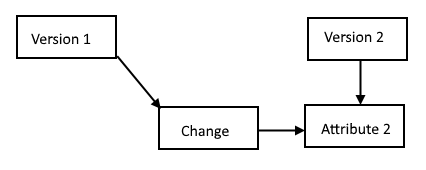
\includegraphics{figures/Addition.png}
	\begin{tikzpicture}[every node/.style={draw, rectangle}]
	\begin{scope}[node distance=20mm and 20mm]
	\node (c) [scale=1.25] at (1,0) {Change};
	\node (1) [above left=of c, scale=1.25] {Version 1};
	\node (2) [above right=of c, scale=1.25] {Version 2};
	\node (a1) [below =of 1, scale=1.25] {Attribute 1};
	\node (a2) [below =of 2, scale=1.25] {Attribute 2};
	
	\draw [line width=2pt,->] (a1) -- (c);
	\draw [line width=2pt,->] (a2) -- (c);
	\draw [line width=2pt, ->] (1) -- (a1);
	\draw [line width=2pt, ->] (2) -- (a2);
	\draw [line width=2pt,->] (c) -- (1);
	\draw [line width=2pt,->] (c) -- (2);
	\end{scope}
	\end{tikzpicture}
	\caption{Highly connected model of just versions, changes, and attributes}
	\label{DiscardedFig4}  % the \label command comes AFTER the caption
\end{figure}
The model addresses the attribution problem by forming two attributes, each associated with a different version.
These attributes inform a change which acts upon both version concepts.
The Log object is dropped for the model since it is a method to convey change and not an actor involved in the change.
From the highly connected construction, new and old attributes no longer need to be explicitly stated, but they can be implied from the model's structure.
A new attribute would not exist in Version 1 so Attribute 1 and its associated properties (arrows) are removed, leaving a unique construction implying an attribute addition.

One observation is that the relation from changes to versions is redundant since the links from version to attribute to change implies the same relationship.
Removing the explicit relation would shorten the number of triples required to encode a change and improve scalability.
The versioning graph using this highly connected model would also be easier to query if the edges were oriented in the same direction, additionally implying that change flows from one version to the next.
These final observations result in the current versioning model.

\subsection{Model Objects}

The versioning model incorporates three kinds of objects: \textbf{versions}, \textbf{attribut\-es}, and \textbf{changes}.
A \textbf{version} object represents the items being compared such as a book or spreadsheet.
In PROV, a \textbf{version} would likely correspond with the \textit{prov:Entity} involved in a \textit{prov:wasRevisionOf} property.
The \textbf{attribute} object refers to specific parts which make up a \textbf{version}.
\textbf{Attributes} could be lines in a book or columns in a spreadsheet.
Including \textbf{attributes} addresses the lack of detail involved in a \textit{prov:wasRevisionOf} or \textit{pav:previousVersion}.
The relationship between \textbf{versions} and \textbf{attributes} captures the influence that changes in the underlying part will have on the overarching \textbf{version}.
Because the model refers to specific parts of a \textbf{version}, the \textbf{version} concept corresponds most closely with a FRBR \textbf{manifestation} rather than an \textbf{expression}.
The presence or absence of an \textbf{attribute} is used to determine the kind of \textbf{change} which occurs to the \textbf{attribute} between \textbf{versions}.
\textbf{Changes} are used to link together \textbf{attributes} from different \textbf{versions}.
The \textbf{change} captures a difference between the old \textbf{version} state and the new \textbf{version} state.
While the \textbf{change} object greatly resembles a PROV qualified property, its form can change depending on the kind of \textbf{change}, like a \textit{schema:UpdateAction}.

\subsubsection{Left-hand Right-hand Convention}

In the following diagrams and figures, the original or base version and its attributes will be placed on the left-hand side and the new version will be placed on the right-hand side with its attributes.
References to the versions as previous and next are avoided since sequencing may not play a major role in distinguishing versions.
Scientific data in large repositories often track sequential releases of data, but a book may have different versions distinguished by printed language.
To recognize this distinction, objects will be referred to as the left-hand \textbf{version} or left-hand \textbf{attribute} when they are not sequentially or temporally related.

\subsection{How Changes are Represented in the Model}

The model bases \textbf{changes} around the three core versioning operations because their commonality across systems provides a fundamental basis for comparisons.
\textbf{Additions} occur when an \textbf{attribute} appears only in the right-hand \textbf{version}.
When an \textbf{attribute} only shows up in the left-hand \textbf{version}, the model captures this as an \textbf{invalidation}.
Finally, a \textbf{modification} change has \textbf{attributes} in both the left and right-hand \textbf{versions}, but it only connects two \textbf{attributes} if their values are different.
These three combinations cover the possible situations within the model.

\begin{figure}
	\centering
	\vspace{0.0in} % normally the command here would be \includegraphics
	%	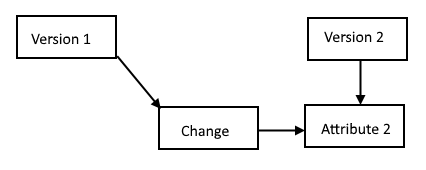
\includegraphics{figures/Addition.png}
	\begin{tikzpicture}[every node/.style={draw, rectangle}]
	\begin{scope}[node distance=20mm and 20mm]
	\node (c) [scale=1.25] at (1,0) {Change M};
	\node (1) [above left=of c, scale=1.25] {Version 1};
	\node (2) [above right=of c, scale=1.25] {Version 2};
	\node (a1) [below =of 1, scale=1.25] {Attribute 1};
	\node (a2) [below =of 2, scale=1.25] {Attribute 2};
	
	\draw [line width=2pt,->] (a1) -- (c);
	\draw [line width=2pt,->] (c) -- (a2);
	\draw [line width=2pt, ->] (1) -- (a1);
	\draw [line width=2pt, ->] (2) -- (a2);
	\end{scope}
	\end{tikzpicture}
	\caption{Model of the relationships between Versions 1 and 2 when modifying Attribute 1 from Version 1 as a result of Change M, resulting in Attribute 2 from Version 2}
	\label{ModificationFig}  % the \label command comes AFTER the caption
\end{figure}

\subsubsection{Modification}

The \textbf{modification} relation occurs when an \textbf{attribute} appears in both \textbf{versions} and their values are different.
In Figure \ref{ModificationFig}, a \textbf{modification} is captured between two versions.
Each \textbf{version} has an \textbf{attribute}, Attribute 1 and Attribute 2, respectively.
Finally, a \textbf{change} object connects the two \textbf{attributes}, denoting that the values described by the attribute are different.

The specific values pertaining to Attribute 1 and Attribute 2 are not captured by the model because acknowledging that a difference exists is more important.
Extending the model to properly communicate the significance of a modification for a wide variety of domains would require sizable domain knowledge and would be outside the scope for this project.
In addition, the model would essentially begin storing a copy of the data set, leading to space and redundancy concerns.

\subsubsection{Addition}

In Figure \ref{AdditionFig}, the \textbf{addition} model differs from the \textbf{modification} construction by the absence of Attribute 1.
\begin{figure}
	\centering
	\vspace{0.0in} % normally the command here would be \includegraphics
	%	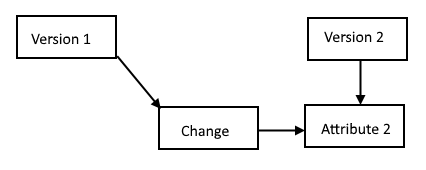
\includegraphics{figures/Addition.png}
	\begin{tikzpicture}[every node/.style={draw, rectangle}]
	\begin{scope}[node distance=20mm and 20mm]
	\node (c) [scale=1.25] at (1,0) {Change A};
	\node (1) [above left=of c, scale=1.25] {Version 1};
	\node (2) [above right=of c, scale=1.25] {Version 2};
	\node (a) [below =of 2, scale=1.25] {Attribute 2};
	
	\draw [line width=2pt,->] (1) -- (c);
	\draw [line width=2pt,->] (c) -- (a);
	\draw [line width=2pt, ->] (2) -- (a);
	\end{scope}
	\end{tikzpicture}
	\caption{Model of the relationships between Versions 1 and 2 when adding an Attribute 2 to Version 2 as a result of Change A}
	\label{AdditionFig}  % the \label command comes AFTER the caption
\end{figure}
The absence creates a disconnect between ``Version 1" and ``Change A".
We know that a connected graph will be desirable to accommodate traversal using linked data query languages so ``Version 1" must be reconnected to the other concepts in the model.
A property is used to create a path between the two \textbf{attributes} to indicate the contribution of  ``Version 1" to the change's lineage.
The path does not show that ``Version 1" informs or creates ``Attribute 2", while that may be true.
The construction was also chosen to create a symmetric orientation with the \textbf{invalidation} change.


\subsubsection{Invalidation}

The \textit{invalidation} model has a missing \textbf{attribute} on the right-hand side of the relation, contrary to the \textbf{addition} construction.
As a result of the invalidation, an attribute no longer exists in the right-hand \textbf{version}.
As seen in Figure \ref{InvalidationFig}, the invalidation change concept matches to the Version 2 object.
\begin{figure}
	\centering
	\vspace{0.0in} % normally the command here would be \includegraphics
	%	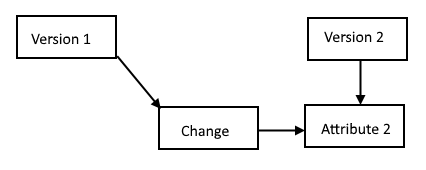
\includegraphics{figures/Addition.png}
	\begin{tikzpicture}[every node/.style={draw, rectangle}]
	\begin{scope}[node distance=15mm and 20mm]
	\node (c) [scale=1.25] at (1,0) {Change I};
	\node (1) [above left=of c, scale=1.25] {Version 1};
	\node (2) [above right=of c, scale=1.25] {Version 2};
	\node (a) [below =of 1, scale=1.25] {Attribute 1};
	
	\draw [line width=2pt,->] (a) -- (c);
	\draw [line width=2pt,->] (c) -- (2);
	\draw [line width=2pt, ->] (1) -- (a);
	\end{scope}
	\end{tikzpicture}
	\caption{Model of the relationships between Versions 1 and 2 when invalidating Attribute 1 from Version 1 as a result of Change I}
	\label{InvalidationFig}  % the \label command comes AFTER the caption
\end{figure}
Just like in \textbf{addition} model, this construction maintains a link between the two \textbf{version} objects.
In this case, it makes more conceptual sense, however, because ``Version 2" invalidates ``Attribute 1" by omitting it.


\section{Encoding a Change Log}

Very little natural language is used in the change log to regularize the format and improve compatibility with RDFa.
The change logs follow a common format with three sections: Additions, Invalidations, and then Modifications.
The sections may be further grouped by column or row additions.
The division means that changes are not published into the change log as they are found, but instead organized and grouped beforehand.

Employing RDFa means that the document must be written using HTML formatting.
Listing \ref{rdfa_list} shows the text necessary to layout the first four lines of Figure \ref{changelog_zoomed}.
While the content only shows four lines, the underlying markup takes up three and a half times as many lines.
Line 2 states that all following resources will be \textbf{attributes} of Version 1.
Line 3 defines such an \textbf{attribute}.
Lines 5 through 8 define the changes Abswurmbachite undergoes.
Because RDFa allows the statements to be embedded within the content, the triples can appear along with the text they describe.
Lines 11 and 12 define complete triples which do not appear in the visible document.
The lines complete the graph, but must be included in spans because RDFa only allows a single triple within each tag.
Modifying the tags' order so that the spans are unnecessary would cause the visible content to appear in an un-logical order, rendering the document machine-readable but not human-readable.

\begin{lstlisting}[language=HTML, caption=Abswurmbachite RDFa, label=rdfa_list]
<h3>Change Log</h3>
<div about="Version1" rel="vo:hasAttribute">
<div resource="v2:Abswurmbachite" typeof="vo:Attribute">
<span style="font-weight:bold" property="http://www.w3.org/2000/01/rdf-schema#label">Abswurmbachite</span>
<table rel="vo:Undergoes">
<tr  about="ChangeAbswurmbachite12" typeof="vo:Change">
<td align="right" rev="vo:Undergoes" resource="v1:AttributeAbswurmbachite12v1" typeof="vo:Attribute"> 9</td>
<td property="vo:resultsIn" resource="v2:AttributeAbswurmbachite12v2" typeof="vo:Attribute">(12)</td>
<td>          </td>
<td>       0.0</td>
<span about="Version1" property="vo:hasAttribute" resource="v1:AttributeAbswurmbachite12v1"></span>
<span about="Version2" property="vo:hasAttribute" resource="v2:AttributeAbswurmbachite12v2"></span>
</tr>
</table></div></div><br>
\end{lstlisting}

After encountering the limitations of using RDFa to include the versioning graph into the change log, JSON-LD was used.
The new format does not rely on the structure of visible content to determine the syntax triples use to be included in the change log.
Listing \ref{json_list} provides the alternative encoding of the Abswurmbachite entry from RDFa.
The entry is significantly longer, almost three times longer than the RDFa entry and ten times longer than the original visible content.
Instead of including all the data in the beginning or end of the document, each change block is separated into the particular \textit{div} section for that change.
This choice allows consumers to extract pertinent change information without needing to ingest the entire versioning graph.

\begin{lstlisting}[language=HTML, caption=Abswurmbachite JSON-LD, label=json_list]
<h3>Change Log</h3>
<div about="v1:Abswurmbachite">
<span style="font-weight:bold" property="http://www.w3.org/2000/01/rdf-schema#label">Abswurmbachite</span>
<table>
<tr  id="ModifyChangeAbswurmbachite12">
<td align="right"> 9</td>
<td >(12)</td>
<td>          </td>
<td>       0.0</td>
<script type="application/ld+json">
[
{
"@context": "https://orion.tw.rpi.edu/~blee/provdist/GCMD/VO.jsonld", 
"@id": "http://CUdb.com/v1/AttributeAbswurmbachite9", 
"@reverse": {
"hasAttribute": "Version1"
}, 
"@type": "vo:Attribute", 
"label": "Primary", 
"undergoes": "http://orion.tw.rpi.edu/~blee/provdist/CU/DTDI/CUjsonlog.html#ModifyChangeAbswurmbachite12"
}, 
{
"@context": "https://orion.tw.rpi.edu/~blee/provdist/GCMD/VO.jsonld", 
"@id": "http://orion.tw.rpi.edu/~blee/provdist/CU/DTDI/CUjsonlog.html#ModifyChangeAbswurmbachite12", 
"@type": "vo:ModifyChange", 
"resultsIn": "http://CUdb.com/v2/AttributeAbswurmbachite12"
}, 
{
"@context": "https://orion.tw.rpi.edu/~blee/provdist/GCMD/VO.jsonld", 
"@id": "http://CUdb.com/v2/AttributeAbswurmbachite12", 
"@reverse": {
"hasAttribute": "Version2"
}, 
"@type": "vo:Attribute", 
"label": "Primary"
}
]
</script>
</tr>
</table></div><br>
\end{lstlisting}

The change logs created with RDFa or JSON-LD demonstrates progress towards documents which are both human and machine-readable.
The implementation provides evidence that JSON-LD is better suited to embed a versioning graph into a change log than RDFa.
RDFa suffers limitations since it is constrained by the content's structure.
The \textbf{modify} relation presented in Figure \ref{NobleGraph1} is unbalanced and the right-hand side of ``ChangeCAM00111" links only to the column \textbf{attribute} but not to the corresponding row \textbf{attribute}.
This stems from a mismatch between the model's structure, the order in which data appears in the change log, and the way RDFa links properties together.
Because the row label forms the outermost encapsulation, it cannot instantiate both row identifiers and implicitly link them separately.
To do so would require explicitly instantiating the \textbf{attribute} in a non-visible part of the document, defeating the purpose of using RDFa to implicitly encode the versioning graph into the document.

Both structured data implementations break up the graph across \textbf{attributes} so that individual parts of the graph can be extracted.
The practice of a one-node JSON object is generally helpful for many web applications to load data quickly, but since the change log is not an application, it makes more sense to break up the content.
Changes to individual \textbf{attributes} can be identified using anchors on the web page, then agents need only extract and parse the linked data to these specific entries.
This way, a subgraph of only the pertinent attributes can be created without first ingesting the entire versioning graph.

An unexpected challenge with the change logs is the larger file size and difficulties in loading the Noble Gas data set's JSON-LD change log.
The problem results from needing ten lines to express a single row in the change log.
Noble Gas also had an impressive number of \textbf{modifications}, some of which are shared across all rows in the data set.
Repeated modifications over rows would account for the explosion in entries within the change log.

\section{Earth Observing Laboratory}



\section{Change Log Analysis}

With a trade-off of 14 HTML lines for every visible line and 40 HTML code lines to each visible line, space utilization is a very present concern.
Table \ref{table:Ng_changelog_table1} shows the size of each encoding of the change log as well as the percentage in size as compared to either of the files involved in the version transition.
\begin{table}
	\caption{Noble Gas change log size: 1st Transition}
	\label{table:Ng_changelog_table1}
	\centering
	\begin{tabular}{|c|r|c|c|}
		\hline
		Encoding Type & File Size (Bytes) & \% of File 1 & \% of File 2 \\
		\hline
		Text&	5575405&	207.8294&	204.2976\\
		RDFa&	62175478&	2317.660&	2278.2745\\
		Turtle&	80919783&	3016.375&	2965.1156\\
		JSON-LD&	130134071&	4850.893&	4768.4577\\
		\hline
	\end{tabular}
\end{table}
`Text' denotes the encoding control where no structured data is included into the change log.
Alone, the control is already double the size of either file.
The RDFa encoding more than 20 times the size of the original files, exceeding the size of the control by more than 10 fold.
A separate file was generated in turtle format to observe whether taking just the linked data values would reduce the information to a more manageable size, but the turtle file was still 30 times the size of the original files.
Adopting the versioning model and encoding it into a change log will very likely require significant storage investment.

Table \ref{table:Ng_changelog_table2} shows the change log sizes for the second version transition in the Noble Gas data set.
\begin{table}
	\caption{Noble Gas change log size: 2nd Transition}
	\label{table:Ng_changelog_table2}
	\centering
	\begin{tabular}{|c|r|c|c|}
		\hline
		Encoding Type & File Size (Bytes) & \% of File 2 & \% of File 3 \\
		\hline
		Text&	670827&	24.5808&	15.9092\\
		RDFa&	6409540&	234.8625&	152.0074\\
		Turtle&	4521010&	165.6618&	107.2194\\
		JSON-LD&	9834772&	360.3721&	233.2396\\
		\hline
	\end{tabular}
\end{table}
Notice that the second transition has much smaller text encodings compared to the original files.
The RDFa and JSON-LD encodings once again 10 and 15 times, respectively, the size of the text encoding.
The turtle encoding, however, is smaller than the RDFa encoding, but still 16 times the size of the original file.
Looking at Table \ref{table:Ng_turtle}, the second transition had 20 times fewer \textbf{Modify} entries, leading to a much smaller turtle file.
\begin{table}
	\caption{Noble Gas Turtle files}
	\label{table:Ng_turtle}
	\centering
	\begin{tabular}{|c|c|c|c|c|}
		\hline
		Filename&	Add&	Invalidate&	Modify&	Total Triples\\ \hline
		changelog.ttl&	608&	216&	102830&	110602\\
		changelog2\_3.ttl&	990&	24&	5369&	8146\\
		\hline
	\end{tabular}
\end{table}

Another way to evaluate the performance of the change log is to look at the number of change entries compared to the number of changed values, in the Copper database's case spreadsheet cells.
From Table \ref{table:Cu_changelog_table1}, the behavior of the encodings is very similar to the second transition of Noble Gas.
\begin{table}
	\caption{Copper change log size: 1st Transition}
	\label{table:Cu_changelog_table1}
	\centering
	\begin{tabular}{|c|r|c|c|}
		\hline
		Encoding Type & File Size (Bytes) & \% of File 1 & \% of File 2 \\
		\hline
		Text&	140131&	41.3152&	59.9580\\
		RDFa&	2032823&	599.343&	869.787\\
		Turtle&	1538772&	453.680&	658.396\\
		JSON-LD&	3500067&	1031.93&	1497.57\\
		\hline
	\end{tabular}
\end{table}
The text format is smaller than the original data set, but the encoded files are at least 10 times the size of the database files.
To determine the number of cells affected by a change, the number of cells added by new rows is summed with the number of cells added by new columns, using the width and length of file 2.
The cells affected by removals is based on the length and width of the first file.
The number of remaining cells, equivalent between the two files is 23940.
Since \textbf{Modifications} are reported cell-by-cell, the number of cells affected is equal to the number of \textbf{Modifies}, 2628.
The rows and columns that \textbf{Modify} affects are not available because the changes appear inconsistently across the rows and columns meaning a reported value would be misleading.
The complete counts are reported in Table \ref{table:Cu_cells}.
\begin{table}
	\caption{Changes to Copper Data}
	\label{table:Cu_cells}
	\centering
	\begin{tabular}{|c|c|c|c|}
		\hline
		Change Type&	Rows&	Columns&	Cells Affected\\ \hline
		Add&	1&	16&	10995\\
		Invalidate&	21&	2&	2145\\
		Modify&NA&NA& 2628\\
		\hline
	\end{tabular}
\end{table}

The triples used to explain changes as a percentage of the cells affected is reported in Table \ref{table:Cu_change}.
\begin{table}
	\caption{Change capture efficiency in Copper Data}
	\label{table:Cu_change}
	\centering
	\begin{tabular}{|c|c|c|}
		\hline
		Change Type&	Triples&	\% of Cells Affected\\ \hline
		Add&	17&	0.065\%\\
		Invalidate&	23&	1.1\%\\
		Modify&	2628&	100\%\\
		\hline
	\end{tabular}
\end{table}
Smaller percentages indicate a higher efficiency of each triple since one triple can explain changes to multiple cells.
Notice that \textbf{Adds} are much more efficient in explaining changes than \textbf{Invalidates} due to the kind of change each triple explains.
\textbf{Invalidates} explained changes to rows primarily while \textbf{Adds} mostly explained changes to columns, but since columns are much longer, \textbf{Adds} ended up scoring higher on efficiency.
\textbf{Modify} triples are extremely inefficient and also account for more than a majority of the changes to the data, meaning that \textbf{Modify} triples most likely account for the bloat in the physical representation of the triples.
Not represented in the change log are the unmodified cells which account for 89.02\% of the matching cells between the Copper files.
The analysis indicates that while \textbf{Add} and \textbf{Invalidate} may be very efficient in expressing changes, improvements to encoding and \textbf{Modify} capture efficiency are needed to bring down the storage costs of automated change logs.
The bloated change log size likely explains the dearth of data set change logs in practice since using the storage space for more data would be more valuable. 

\section{Summary}

The automated change log generation yielded some unexpected results.
Automated change logs standardize the process to capture change within a data set.
While more popular text-only change logs could be adopted, a versioning data model was necessary to make the logs also machine computable.
The computability improves user navigation over large data sets.
The drawback is that the encoded change logs are reliably much larger than the original data set in bytes.
The storage space cost likely contributes to the reason that change logs are often unseen in data set documentation.
The automation and inclusion of change logs inform consumers how much the data set has changed.

The versioning model provides a method to capture change information in greater detail than current provenance models.
The inclusion of \textbf{versions} and \textbf{attributes} into the model connect changing items with the objects they influence.
The \textbf{changes} create a ladder-like structure to connect together \textbf{version} objects in greater detail.
Each rung of the ladder can not only be counted, but also grouped into types of change according to the respective operation.
The method of instantiating a versioning graph will be covered in Chapter \ref{ch:graph}.

The human-readable presentation defines the structure which tags in the chan\-ge log must take since maintaining human-readability is desired.
The structure then determines the order in which linked data statements must appear in the log to encode the graph with RDFa.
The ordering creates limitations on how strictly the encoded graph adheres to the specification from Chapter \ref{ch:model}.
While construction of the change log is automated, encoding through RDFa significantly reduces the source HTML readability.
In other applications using RDFa, the triples describe and link the text encapsulated by HTML tags.
The versioning graph exclusively ignores the marked up content and links together tags or explicitly defines full triples in span tags.

Change logs are much less restricted when encoded using JSON-LD rather than RDFa.
The encoding format pulls the graph out of the attributes where they do not interact with content and into a separate script section.
The method causes a drastic expansion per change in necessary text.
The decision to divide up JSON-LD objects by the row in the change log they describe likely contributes significantly to the overhead necessary for the encoding.
The division was made with the forethought that change log consumers may desire to only ingest specific subgraphs of the versioning graph.
Separated JSON-LD objects will likely need to be merged in the future to save space for data sets with many changes.

The resulting logs end up very large and sometimes do not load in a browser.
Reassuringly, both data sets displayed the same space usage complexity with RDFa being ten times the plain text size and JSON-LD twice the size of a change long in RDFa.
The relationship unfortunately means that a JSON-LD change log, with more readable source code, is twenty times the size of a plain text change log.
The Copper data set's logs were reasonably responsive, displaying in seconds, but the Noble Gas's change log did not.
In order to retain usability, there will need to be methods optimizing change log structure or representation.